\documentclass[pdftex,12pt]{artikel3}
% Compile with:  pdflatex 

% Settings for source listings.
\usepackage[dvips,letterpaper,margin=1.1in]{geometry}
\usepackage{listings,graphicx}
\usepackage{url}    % usage \href{}{}
\usepackage{xcolor}
%% \usepackage{soul}
%% \usepackage{lipsum}
\usepackage{mathtools}
% \newcommand{\myul}[2][black]{\setulcolor{#1}\ul{#2}\setulcolor{black}}
\usepackage{array}
%% \usepackage{multirow}
\usepackage{alltt}
\usepackage{pifont}
\usepackage{fancyvrb}
\usepackage{enumitem}
\usepackage[hidelinks]{hyperref}   % hide links in hyperref text
\usepackage{cleveref}     % nice table/figure refs. put after hyperref

% sample stuff for tables and figs
%\usepackage{blindtext}

\usepackage{makeidx}      % for makeindex
\usepackage{tocloft}      % for nicely formatted toc, tof, lof
\usepackage{booktabs,longtable,tabu}

\usepackage[utf8]{inputenc}
\usepackage[T1]{fontenc}
\usepackage{imakeidx}
%% preamble

% the tabfigref command outputs a table or figure reference
% with pattern: "Figure N, The Caption," or "Table N, The Caption,"
% Note: output has a trailing comma(,) for phrasing.
\newcommand{\tabfigref}[1]{\autoref{#1}, \nameref{#1},}

\setcounter{tocdepth}{3}
\makeindex[columns=2, title=Alphabetical Index, intoc]

\lstset{tabsize=4,language=Python,showstringspaces=false}

\title{
\begin{center}
\huge{Jupyter Notebook User Document} \\
\huge{CSCI-471-02}\\
\end{center}
\\
\\
\\
\\
\\
\author{} % \author{Jeffery B. Russell} \\
          % \author{Daniel Moore}
\date{}   % \date{Febuary 20, 2020} 
}

%% document starts
\begin{document}
\maketitle


\begin{center}
\author{Jeffery B. Russell}
\author{Daniel Moore}
\author{Lauden Y}

\date{Febuary 20, 2020}
\end{center}

\newpage

\tableofcontents
\addtocontents{toc}{~\hfill\textbf{Page}\par}
\addcontentsline{toc}{section}{\listfigurename} % include lists of figs
\newpage
\listoffigures
\addtocontents{lof}{~\hfill\textbf{Page}\par}

\newpage

\section{Introduction}

Jupyter Lab is an open-source web-based notebook tool that you can use as your development environment.
A coding notebook enables you to intermix markdown, and code blocks that you can execute in a single document. This is heavily used in the education and research fields because it makes writing reports easy and reproducible. With Jupyter you can create content that has live code, equations, visualizations and explanatory text. 

Applications of Jupyter Jab:

\begin{itemize}
  \item Quick Experimentation
  \item Telling a story with data
  \item Writing a report
  \item Sharing code snippets for education
\end{itemize}

In this document we are going to go over the basic installation and usage of Jupyter Lab for personal use developing python\index{python}. In the advanced usage section we go over how to use 

\section{Installation}

To install, first go to \href{https://jupyterlab.readthedocs.io/en/stable/getting_started/installation.html}{Jupyter Install} for a detailed guide. This user document assumes that you install Jupyter Lab. \textbf{Do Not Install Jupyter Notebook. }

\subsection{Prerequisites}
In order to install Jupyter, you must have Python installed. Your version of Python \textbf{must be 3.3 or greater}. As part of having Python, you will also have pip. Click \href{https://www.python.org/downloads/}{here} for the latest version of Python\\
\\
However, we highly recommend you take the time now to install \href{https://docs.conda.io/projects/conda/en/latest/user-guide/install/}{Conda} now because it'll be helpful later one with some of the more advanced features of Jupyter as well as machine learning focused Python.\\
\\
You should also have either Firefox, Chrome or Safari as these are the only browsers Jupyter is currently known to work with.

\subsection{Installation on Linux}
There a two ways of installing Jupyter on Linux.\\
\\
Using pip the command is \textbf{pip install jupyterlab}.\\
\\
Using conda the command is \textbf{conda install -c conda-forge jupyterlab}

\subsection{Installation on Windows}
Installation on Windows is the same as installation on Linux except that you must also add the user-level bin directory if you installed using \textbf{pip install --user}.

\section{Usage}

To run Jupyter Lab, open your computer's command terminal and enter the following command. This will open Jupyter Lab in your default web browser.

\texttt{jupyter lab}

\tabfigref{fig:jupyterlablauncher} is what you will see upon first running Jupyter Lab. Otherwise, it can open to the most recent notebook you were working on.

\begin{figure}[h!]
    \centering
    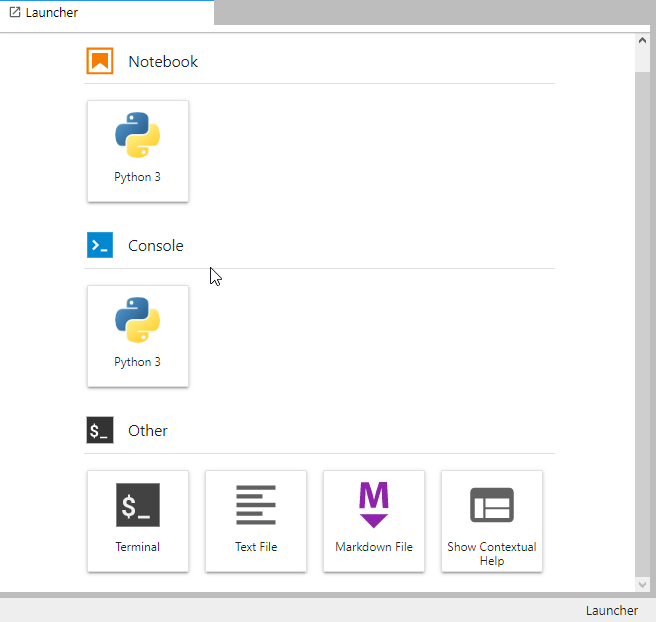
\includegraphics[width=65mm]{launcher.png}
    \caption{Default Jupyter Lab launcher}
    \label{fig:jupyterlablauncher}
\end{figure}

\subsection{Navigation}

Once Jupyter Lab is running, you will see on the left side of the screen a column of icons. Each icon will open a different panel to the right of it when you click it. From top to bottom, these icons have the following functions:

File Browser (folder icon): displays a file browser for the user to open, move, or delete their files.

Running Terminals and Kernels (square stop button inside a circle): shows the user all currently active terminal and kernel sessions.

Commands (palette icon): allows the user to enter various commands into Jupyter Lab.

Notebook Tools (wrench icon): shows various options for the user's current notebook.

Open Tabs (a tabbed window icon): lists all currently open tabs in Jupyter Lab.

Additionally, the top toolbar conta

\subsection{Creating a Notebook}

To create a notebook (the working document for both python code and text markdown) from the launcher (\tabfigref{fig:jupyterlablauncher}), click on the Python 3 icon under the orange notebook symbol. Alternatively, if you don't have the launcher open, you can click on File in the toolbar, click New, and finally click Notebook.

\subsection{Running a Notebook}

\subsection{Exporting Notebooks}
In order to export the document, click the \textbf{File} tab, mouse down to \textbf{Export Notebook As...} and then click any of the myriad of formats to export as that format. 

\subsection{Customization}
Customization of Jupyter is in general exceptionally easy.\\
\\
In order to change the theme, one simply needs to go to the \textbf{Settings} tab and drop down to JupyterLab Theme. This will allow you to change from light to dark mode as well as the font sizes for the code, content and UI.\\
\\
Scrolling down the rest of the Settings you see many other things that can be customized.\\
\\
Advanced settings allows you to customize many aspects of Jupyter Lab such as keyboard shortcuts, terminal settings, and a myriad of others.

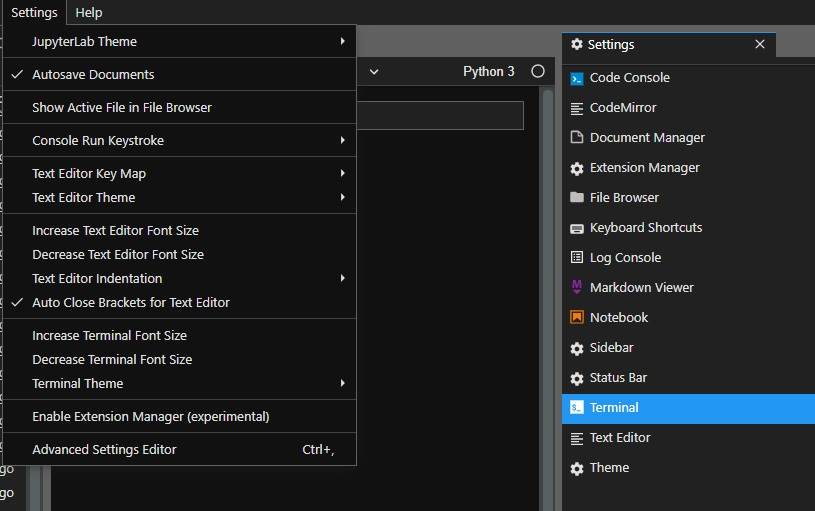
\includegraphics[scale=.6]{Jupyter Settings.jpg}

\section{Advanced Usage}

\subsection{Multiple Kernels}

\subsection{Remote Connection}


\subsection{Running a Server}


\newpage

\section{Glossary}

\begin{itemize}[label={}]
\item {\bf Jupyter}: Nonprofit organization created to "develop open-source software, open-standards, and services for interactive computing across dozens of programming languages". \footnote{{\url https://jupyter.org/}}\index{jupyter}\\
\item {\bf Python}: High-level interpreted, general purpose programming language \footnote{{\url https://www.python.org/}}.\index{python}\\
\item {\bf Markdown(MD)}: Lightweight markup-language \footnote{{\url https://en.wikipedia.org/wiki/Markdown}}.\index{markdown}\\
\item {\bf pip}: Tool for installing and managing python packages \footnote{{\url https://pypi.org/project/pip/}}.\index{pip}\\
\item {\bf Scala}: General purpose functional programming language that runs on the JVM \footnote{{\url https://scala-lang.org/}}.\index{scala}\\
\item {\bf R}: Programming language for statistical computing and graphics \footnote{{\url https://www.r-project.org/}}.\index{r}\\

\end{itemize}

\newpage

\section{References}

\begin{enumerate}
\item
{\url https://en.wikipedia.org/wiki/Finite-state\_machine}
\item
TODO
\end{enumerate}

\newpage

\section{Index}
\printindex
% outputs its own heading, which does not match the sections

\end{document}